\subsection{Hardware suggestion}
\label{sec:hardware-suggestion}
	The following section of this report describes the hardware and software suggestion for interfacing with the \texttt{MIC-2 MKII's} modbus interface. The hardware/software stack should be able to readout several registers of the device over modbus. Then the data should be sent via \ac{MQTT} to a broker within the THM network for further processing and visualization.

	\subsubsection{Development board}
		As the microcontroller development-board was picked the \texttt{OLIMEX ESP32-GATEWAY} board. Olimex is a provider of development boards, embedded device programmers and other development tools.~\cite{olimex}
		The board itself is depicted within \cref{subfig:hw-components} on the left side. The following list gives a brief overview about the features of this development board.
		\setlist{noitemsep}
		\begin{itemize}
			\item ESP32-WROOM32 module
			\item CH340B USB-UART converter for programming
			\item Ethernet 100MB interface (LANA710A phy chip)
			\item MicroSD card slot
			\item 20-Pin GPIO connector with all ESP32 ports
		\end{itemize}
		\begin{figure}[H]
			\subfloat[OLIMEX ESP32-GATEWAY]{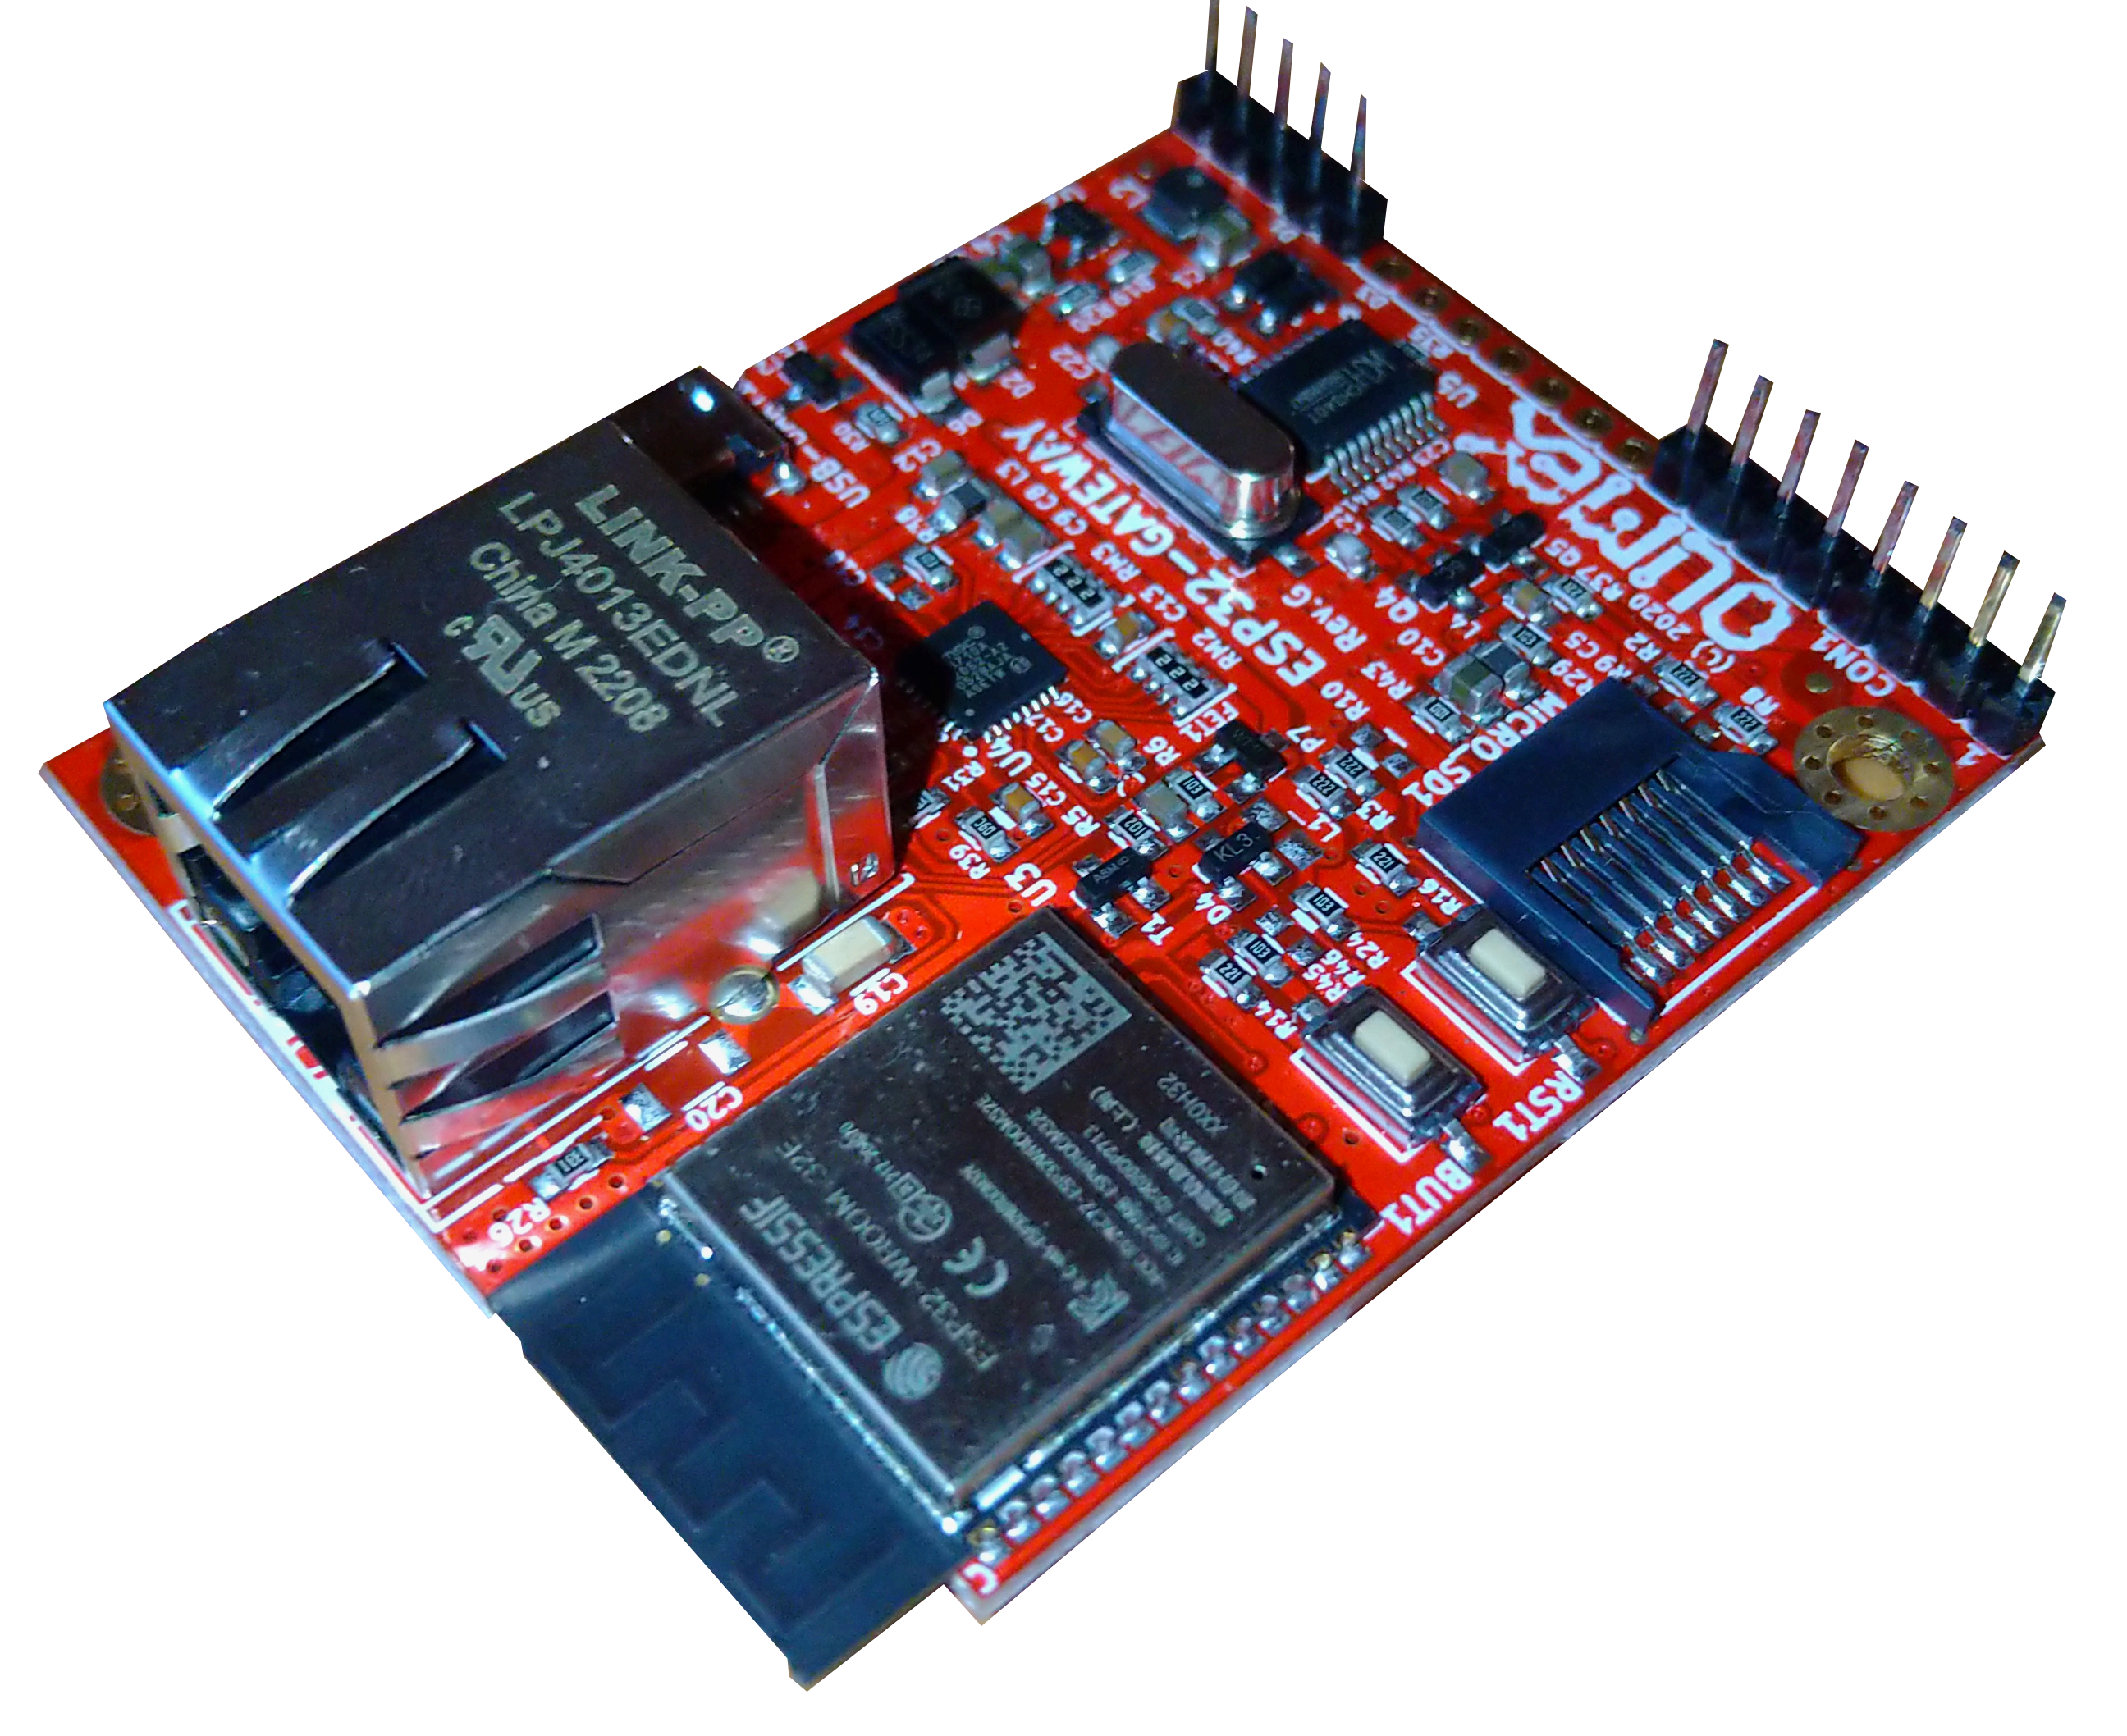
\includegraphics[width=0.5\linewidth]{assets/RD-esp32-gateway.png}}\qquad
			\subfloat[RS485 module~\cite{IMG-rs485conv}]{\includegraphics[width=0.5\linewidth]{assets/RD-rs485-converter.png}}
			\caption{Selected hardware for connection with \texttt{MIC-2 MKII}}
			\label{subfig:hw-components}
		\end{figure}
			The board seems to be well suited for this application because it's quite cheap with an average price of $ 16.59 € $ (in 11/01/2023) and has an onboard ethernet transceiver and port. The ethernet port was one of the main criteria when picking the board because wireless communication form inside the wiring closet, where the device should be placed, might not be a good choice for reliable communication. The onboard \texttt{CH340B} chip brings the advantage to easyly flash the board without an externel \ac{USB} to \ac{UART} converter. This gives more flexiblity when developing the firware for the board. The onboard sdcard is not really necessary in the context of this work.\\ %TODO: ggf beschreiben dass man werdte puffern kann
			At least there is one other advantage to mention here: The board has open-source hardware, so the schematics can be freely browsed in the internet.
	\subsubsection{RS485 interface}
		The pickd RS485 interface is depicted in \cref{subfig:hw-components} on the right hand. The module then connects to the development board with $ 3.3~\si{\volt} $ supply voltage and ground. The \texttt{TXD} and \texttt{RXD} pins connect the \ac{UART} interface between the board and the converter. On the right edge of the converter module you can see the \texttt{A+} and \texttt{B-} pins which later will be connected to the modbus device. They communicate over RS485 levels. Unfortunately the chip on the converter was milled of so that it was impossible to lookup the \ac{IC} used on those types of boards.
		
		\begin{figure}[H]
			\includegraphics[width=\linewidth]{assets/RD-esp-rs485-hw-conn.pdf}
			\caption{Schematic of connection between ESP32-GATEWAY board and the RS485 converter}
			\label{fig:gw-converter-hwconn}
		\end{figure}
		
		The precedent \cref{fig:gw-converter-hwconn} outlines the wired connections between the UART to RS485 converter used in this project with the ESP32-GATEWAY board. For mounting and installing those two connected boards in the wiring cabinet it will aditionally be necessary to design an enclosure. This will be further described in TBD.%TODO: cref auf kapitel mit 3d gehäuse!
		The GPIO-Pins $ 4 $ and $ 13 $ were chosen because they aren't occupied by specific hardware functions already present on the development board (e.g. SD-Card slot). One additional challange was not to use pin $ 12 $ because it's a \enquote{strapping} pin. Those pins must be left floating or pulled to ground when flashing the device.
		
	\subsubsection{Case-design}
		For installing the device a kind of case should designed to avoid short-circuits or other damage to the hardware when placing it somewhere. Therefore a very simple base-plate was desgined and 3D printed in order to protect the bottom of the ESP32-GATEWAY's board.
		
		\begin{figure}
			\centering
			\includegraphics[width=0.8\linewidth]{assets/RD-board-mount}
			\caption{ESP32-GATEWAY + RS485 Converter Board mount}
			\label{fig:board-mount}
		\end{figure}
		
		\Cref{fig:board-mount} shows an exported 3D drawing created with the CAD-Application FreeCAD. The real mount was printed on a Prusa Mini+ 3D printer with PLA filament. After mounting the board the bolts were molten with a soldering iron to hold the board in-place. The RS485 Board was glued onto the mount.